Based on our specification we created a design for the application's user interface (UI). The UI had to support the use cases specified in section \ref*{sec:use_cases}, although not all features required in the use cases were included in the design. The goal of the design was to include the features listed as \textit{Must have} and \textit{Should have} in the MoSCoW analysis, but still take the other features into account. This was done to ensure that the most important aspects of the use cases would be satisfied in the design, while also having designed for some of the desirable, but less important features.
In the following sections we describe wireframes each showing a view of a page on our web application. Furthermore, each section will include a description of which use cases and features each page satisfies.

\section{Wireframe for Solving Exercises}
The wireframe in figure \ref{fig:wfExercise} shows the page intended for solving exercises.
% primary use cases
% solve exercises
\begin{figure}[H]
	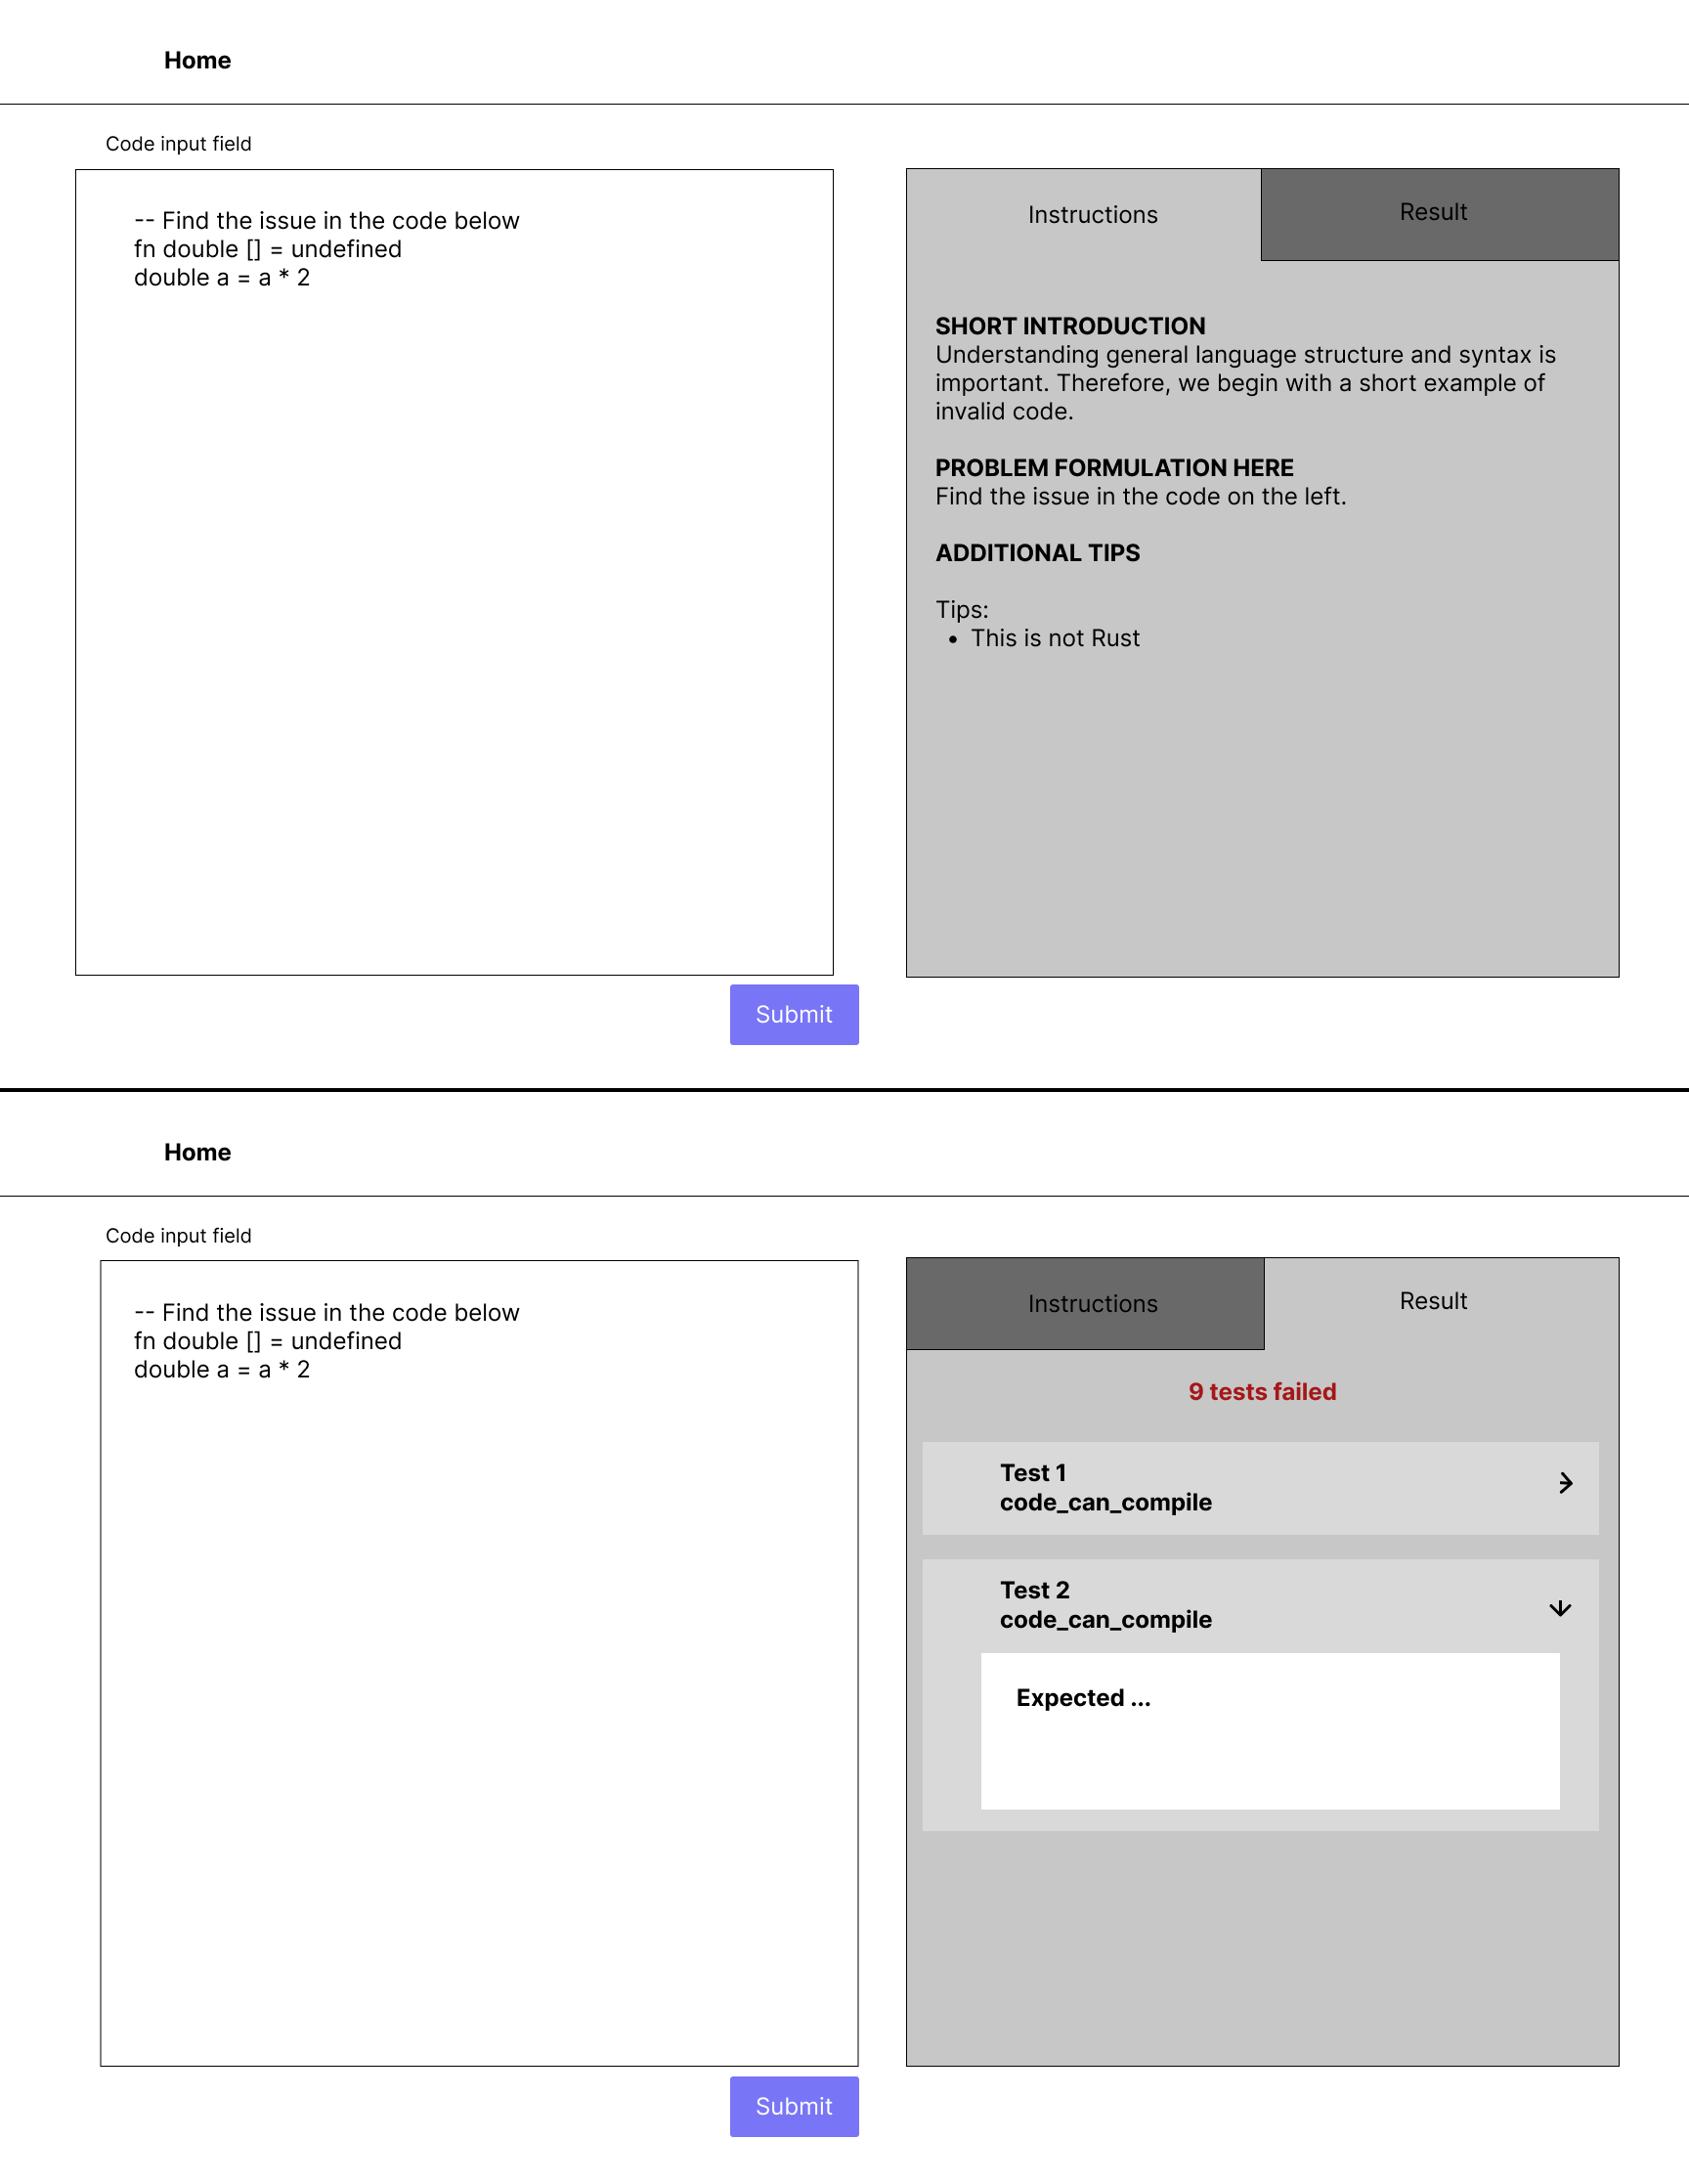
\includegraphics[scale=0.15]{WireframeSolveExercise.png}
	\centering
	\caption{Wireframe for solving an exercise}
	\label{fig:wfExercise}
\end{figure}

For both images in figure \ref{fig:wfExercise} a text input field can be seen located on the left. This text input field is where the user can input code for submission. On the right side of the top image of figure \ref{fig:wfExercise}, a box can be seen containing two tabs. The currently selected tab of this image is the \textit{Instructions} tab which is where the instructions for the current exercise is displayed. On the right side of the bottom image is a similar view, except that the \textit{Result} tab has now been selected. This tab shows the result of the submitted code, whether it passed the tests for the exercise and whether it compiled. This design satisfies the requirements that an exercise should have a description and that a user should be able to submit and verify their code and exercise submission stated in the use case \textbf{Solve exercises}.

\section{Wireframe for Browsing}
The design for the page displayed in figure \ref{fig:wfExercise} does not satisfy the entirety of the use case \textbf{Solve exercises}, as we have designed a separate page to browse exercises as well as sessions and syllabi. The page structure for all of these are similar, and therefore we only show an example of a page for browsing syllabi.
% Structure of creating sessions and syllabi
\begin{figure}[H]
    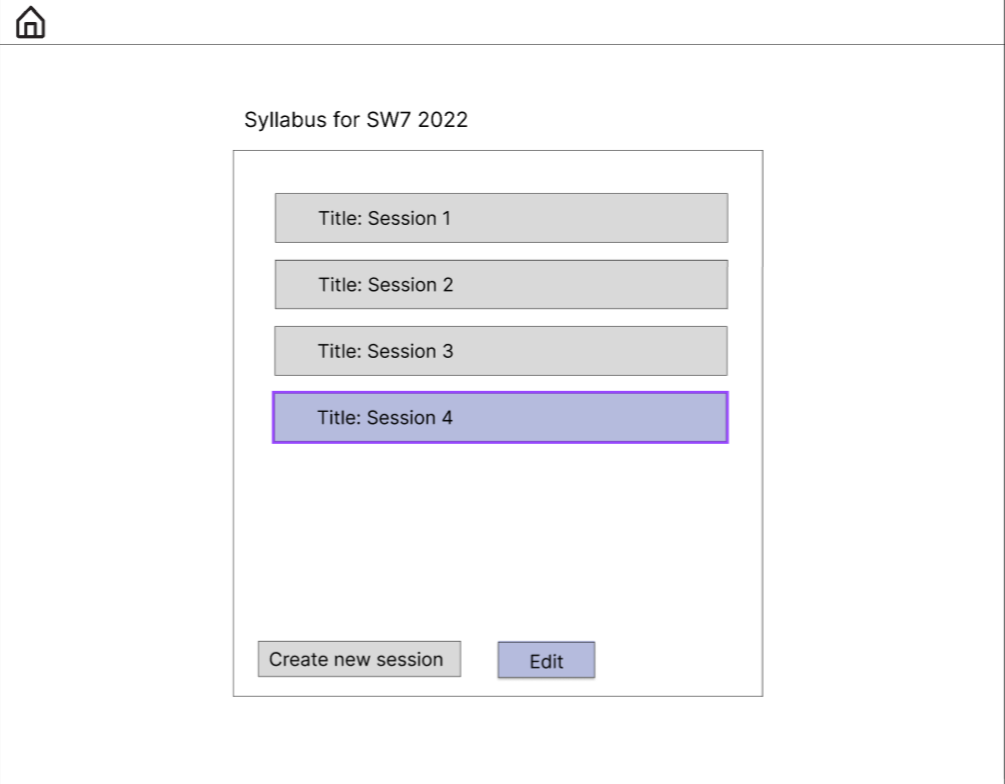
\includegraphics[scale=0.3]{browseSyllabus.png}
    \centering
    \caption{Wireframe for browsing a syllabus}
    \label{fig:wfSyllabus}
\end{figure}
Note that the buttons related to creating new items or updating items in the list will only be available to the lecturer. The items shown in the list corresponds to which page that the user is on. If the user is browsing syllabi, then the items contained in the list will be syllabi. If the user is browsing sessions, the list will contain sessions. Similarly for exercises. This design satisfies the section of the use case \textbf{Solve exercises}, related to choosing sessions and exercises. Additionally, it also satisfies part of the use case \textbf{Create exercises} related to having the ability to create and edit syllabi and exercises.

\section{Wireframe for Creating an Exercise}
The wireframe in figure \ref{fig:wfProblem}, shows the page that the lecturer will see, when the create exercise button when browsing exercises.
% create exercises
\begin{figure}[H]
	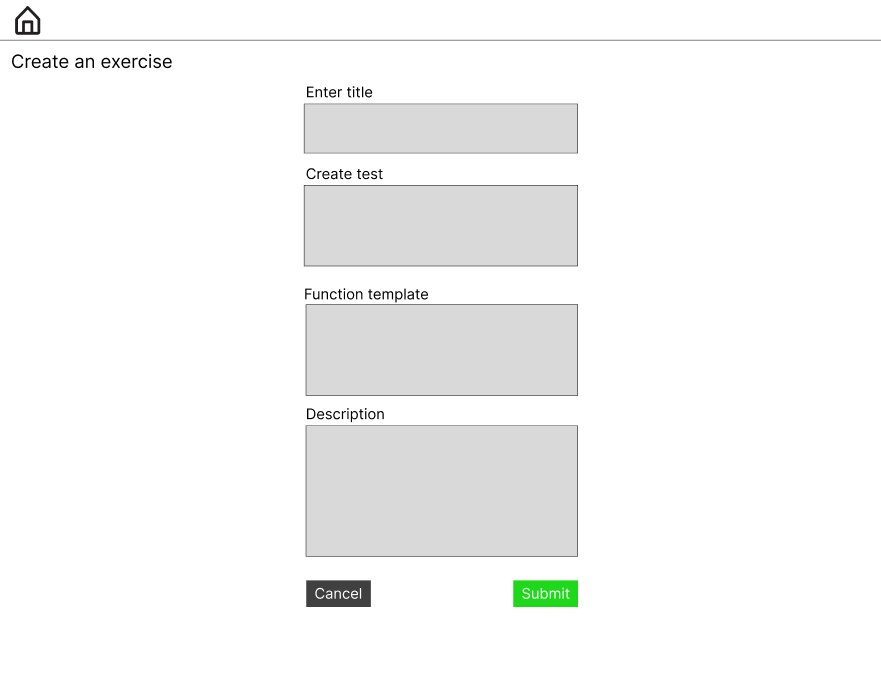
\includegraphics[scale=0.6]{createProblem.jpg}
	\centering
	\caption{Wireframe for creating a problem}
	\label{fig:wfProblem}
\end{figure}

This page allows the lecturer to create an exercise with a title, test, function template and description. These are fields required to provide the information necessary for a student to solve the exercises. Additionally, test field allows a lecturer to specify the tests that student's code must pass. The function template field allows the lecturer to specify functions that the test will call, and which will be included in the editor on the solve exercise page. This satisfies the remaining requirements of the use case \textbf{Create exercises}.